\documentclass{article}
\usepackage{geometry}
\usepackage{graphicx}
\usepackage{float}
\usepackage{subfig}
\usepackage{epsfig}
\usepackage{epstopdf}
\usepackage{amsmath}
\usepackage{commath}
\linespread{1.2}



\title{ECS 271 Homework2}
\date{\vspace{-5ex}}
\begin{document}
\author{Jiahui Guan, Leyuan Wang}
\maketitle
\section{Overview}
Recommender systems can be generated by a wide spectrum of algorithms. Compared with the simple and intuitive user-based or item-based collaborative filtering methods, matrix factorization techniques which discover the latent features underlying the interactions between users and items are usually more effective and commonly used. In this assignment, we are provided with a group of Netflix users and a set of movie items and each user have rated some movies in the system, and we are asked to predict how users would rate the movies that they have not rated yet, such that we can make recommendations to them. This can be formulated as a learning problem in which we are given the ratings that users have have given certain items and are tasked with predicting their ratings for the rest of the items. We try two different methods, SGD(stochastic gradient descent)-based and SVD(singular value decomposition)-based matrix factorization. 

\section{SGD-based Matrix Factorization via Alternating Least Squares (ALS)}
The intuition behind using matrix factorization to solve this problem is that there should be some latent features that determine how a user rate an item. The latent features can be the different categories of movies or the actors/actresses. If we can discover such features, we should be able to predict a rating with respect to a certain user and a certain item. We can assume that the number of features is smaller than the number of movies and users since we admit the fact that at least two movies share a same feature. 

If there are $n$ users and $m$ movies, we are given an $n\times m$ matrix $R$ in which the $(i,j)^{th}$ entry is $r_{ij}$ -- the rating for movie $j$ by user $i$. Matrix $R$ has many missing entries indicating unobserved ratings. Assume that we would like to discover $k$ latent features, where we fix a relatively small number $k$. Our task is then to find two matrices $P$ ($n\times K$ dimension) and $Q$ ($m\times K$ dimension) such that their product approximates $R$:
\[ R \approx P \times Q^T = \hat{R}
\]
Each row of $P$, vector $p_i$, represents the strength of the associations between a user and the features and each row of $Q$, vector $q_j$ represents the strength of the associations between a movie and the features. We formulate this problem as an optimization problem in which we aim to minimize an objective function and find optimal $P$ and $Q$. And we define the objective function as the least square error of the observed ratings and we regularize them:
\[ \underset{P,Q}{min} \sum\limits_{r_{ij}>0}(r_{ij}-p_iq_j^T)^2+\lambda(\sum\limits_i\norm{p_i}^2+\sum\limits_j\norm{q_j}^2 )
\]
The regularization parameter $\lambda$ is used to control the magnitudes of the user-feature and movie-feature vectors such that $P$ and $Q$ can give a good approximation of $R$ without having to contain large numbers. Notice that the objective function is non-convex because of the $p_iq_j^T$ term; it's NP-hard to optimize. Gradient descent can be used as an approximate approach here but it turns out to be slow and costs lots of iterations. However, if we fix the the set of variables $P$ and treat them as constants, the objective function will be a convex function and vice versa. Our approach is therefore to fix $Q$ and optimize $P$, then fix $P$ and optimize $Q$, and repeat until convergence. The approach is known as Algernating Least Squares (ALS). 

We initialize the two matrices $P$ and $Q$ with some random values, caculate the difference of their product compared with $R$ and try to minimize the difference iteratively using back propogation. The difference or error rate between the estimated ratings and the real ratings is as follows:
\[ E^2 = (R-\hat{R})^2+\frac{\beta}{2}(\norm{P}^2+\norm{Q^2}) = (R-PQ^T)^2+\frac{\beta}{2}(\norm{P}^2+\norm{Q^2})
\]
To minimize the error, we need to know in which direction we have to modify the values in $P$ and $Q$. We differentiate the above equation to find the gradient at current values. 
\[
\frac{\partial}{\partial P}E^2 = -2EQ^T=-2(R-\hat{R})Q^T + \beta Q^T\]
\[\frac{\partial}{\partial Q}E^2 = -2EP=-2(R-\hat{R})P +\beta P
\]
We then update $P$ and $Q$
\[
P'= P+\alpha\frac{\partial}{\partial P}E^2 = P+\alpha(2EQ^T-\beta P)\]
\[Q'= Q+\alpha\frac{\partial}{\partial Q}E^2 = Q+\alpha(2EP-\beta Q)
\]
Here $\alpha$ is a constant which determines the stepping rate approaching the local minimum. 

We use the \emph{cudarray} library to implement our method on the GPU to accelerate the computation since GPUs are famous for their high arithmetic compuational power and our matrix computations are embarrassingly parrallel which can be a good fit for GPU computations. And it turns out that our GPU implementation using \emph{cudarray} is much faster and saves us a lot of time to converge compared with the parallel CPU implementation using \emph{numba} package. We attached our code in Section~\ref{code}.  A diagram of our ALS is shown in Figure~\ref{fig:sgd}.
\begin{figure}
  \centering
  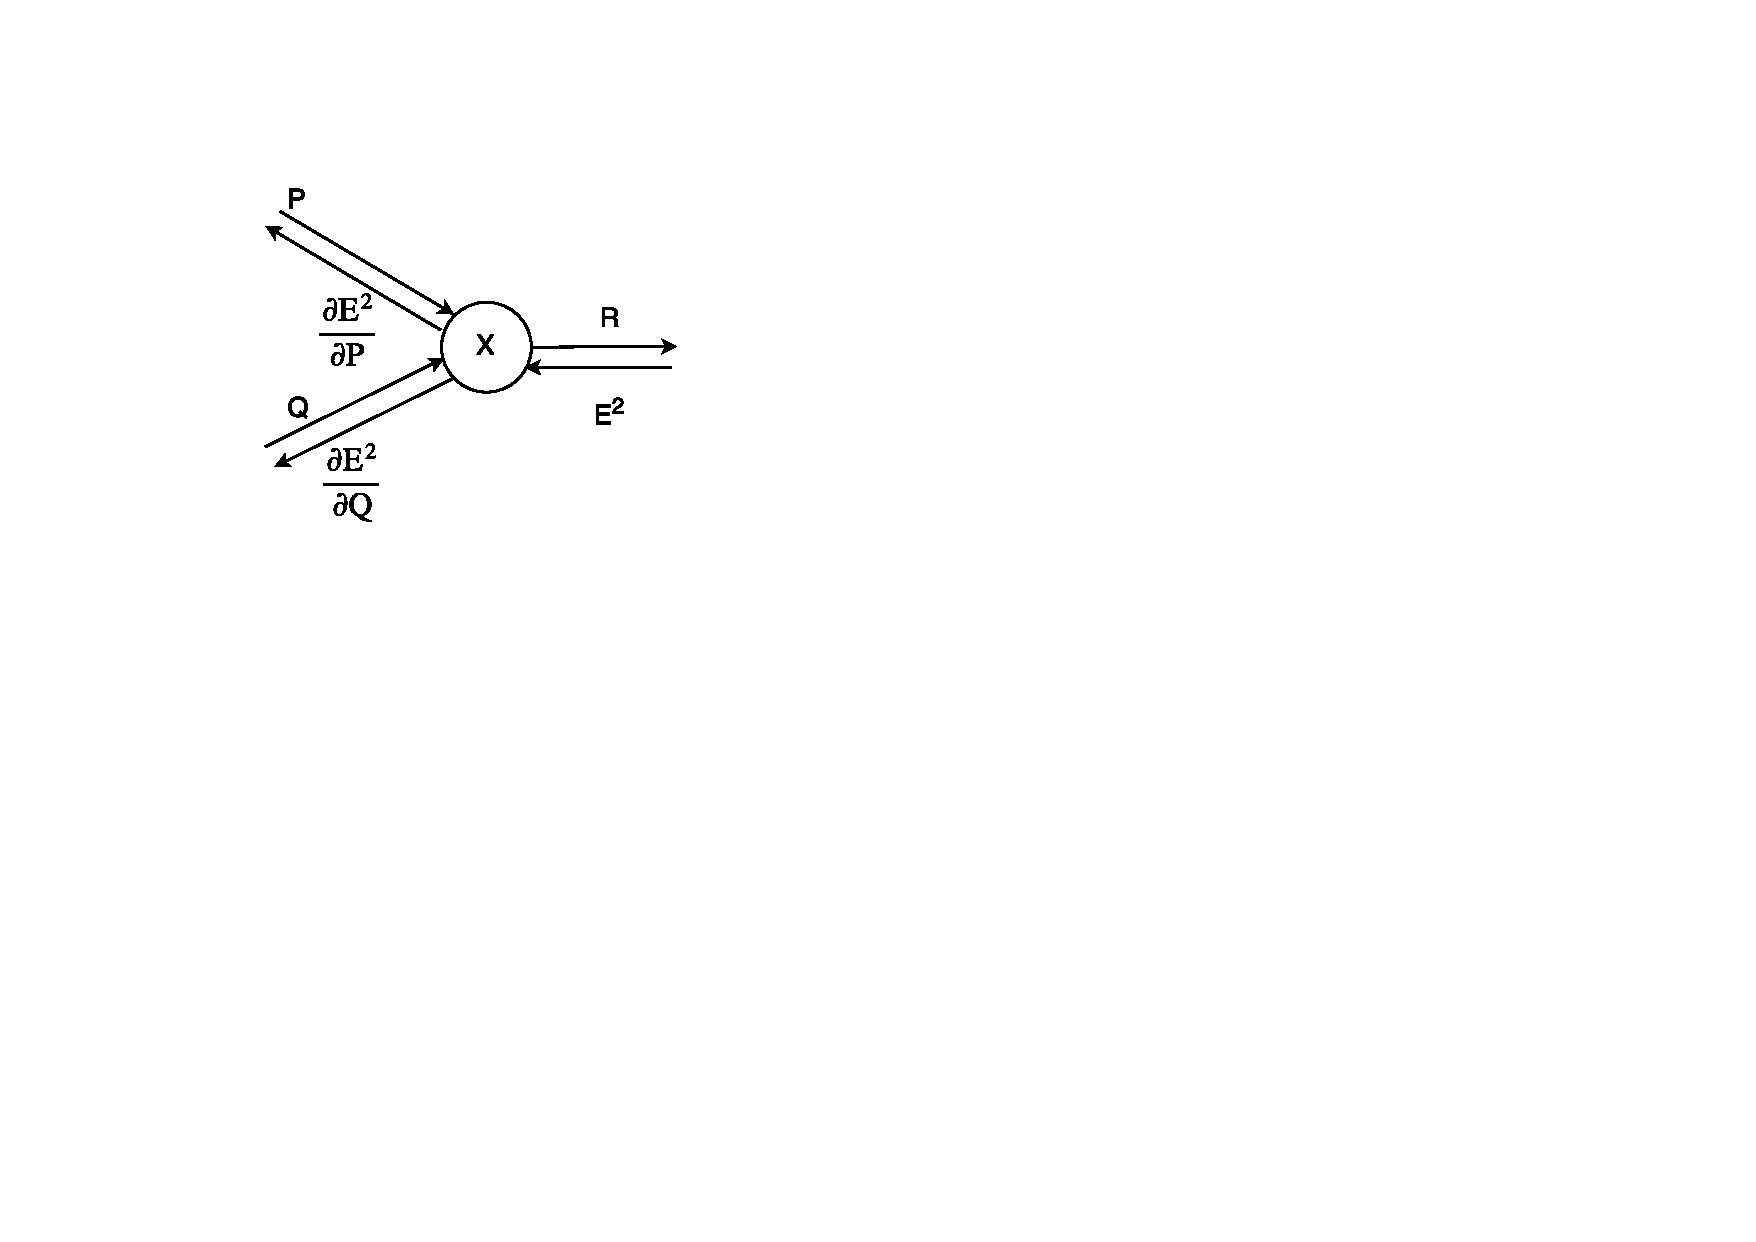
\includegraphics[scale=0.8]{SGD}
  \caption{SGD-based matrix completion diagram.\label{fig:sgd}}
\end{figure}


\section{SVD Method} 
We use Singular Value Decomposition method as our matrix factorization approaches to unsupervised learning. Let $A$ be the training dataset with row ordered as user id and column as movie id. The entries of $A$ will be the rating, a latent variable, from 1-5. We decompose $A$ using SVD, that is, $A=UWV^T$
\begin{equation}
\begin{bmatrix}
&&&\\
&A&\\
&&&\\
\end{bmatrix}=\begin{bmatrix}
&&&\\
&U&\\
&&&\\
\end{bmatrix}
\begin{bmatrix}
w_1&&\\
&\vdots&\\
&&w_n\\
\end{bmatrix}
\begin{bmatrix}
&&&\\
&V&\\
&&&\\
\end{bmatrix}^T
\end{equation}
Where $\begin{bmatrix}
w_1&&\\
&\vdots&\\
&&w_n\\
\end{bmatrix}$ corresponds to the eigenvalues of $A$. \\

Next thing we want to do is the have a good approximation of $A$. The criterian of such aprroximation matrix is that 
\[\min_{X}||A-X||_F: \textbf{rank}(X)=k \]
We set all but the largest $k$ singular values to zero since the other smalle eigenvalues are almost neglectable. So a best $k$-rank approximation $\hat{A}_k$ is given by zeroing out the $r-k$ trailing singular values of $A$, that is 
\[\hat{A}_k=U\hat{S}_kV^T, \hat{S}_k=\textbf{diag}(\sigma_1,...\sigma_k,0,...0)\]

The minimal error is given by the Euclidean norm of the singular values that have been zerored out in the process: 
\[||A-\hat{A}_k||_F=\sqrt{\sigma_{k+1}^2+...+\sigma_{\tau}^2}\]


Here we use Python to implement SVD method. We also use the package \textit{sklearn.utils.extmath} function SVD to get the decomposed matrices. Based on the eigenvalue plots, we set $K=23$ as our 23 largest eigenvalues.


\section{Appendix}
\label{code}
\paragraph{SGD code}
\begin{verbatim}  
try:
    import numpy as np
except:
    print "This implementation requires the numpy module."
    exit(0)

import csv
import scipy.sparse as sparse
import os
os.environ['CUDARRAY_BACKEND'] = 'cuda'
import cudarray as ca

def matrix_factorization(R, P, Q, mask, steps=200000000, alpha=0.00005, beta=0.02):
    Q = ca.transpose(Q)
    for step in xrange(steps):
 	E = ca.subtract(R, ca.multiply(ca.dot(P,Q), mask))

	rmse = ca.sqrt(ca.sum(ca.power(E,2)) / ca.sum(mask))
	rmse = np.array(rmse)[0]

 	print 'step: %i RMSE: %f' % (step, rmse)
        if rmse < 0.65:
            break
	P = ca.add(ca.multiply(P,(1-alpha*beta)),ca.multiply(ca.dot(E,ca.transpose(Q)), 2*alpha))
	Q = ca.add(ca.multiply(Q,(1-alpha*beta)),ca.multiply(ca.dot(ca.transpose(P),E),2*alpha))

    return P, Q
    
if __name__ == "__main__":
    X = np.loadtxt('train.csv', delimiter = ',', usecols = (0,1,2), skiprows = 1)
    Y = np.loadtxt('test.csv', delimiter = ',', usecols = (0,1), skiprows = 1, dtype=int)
    shape = tuple(X.max(axis=0)[:2]+1)
    R = sparse.coo_matrix((X[:,2], (X[:,0], X[:,1])), shape = shape, dtype = X.dtype)
    R = R.todense()
    R = np.array(R)
    mask = np.divide(np.array(R, dtype=int), np.array(R, dtype=int))
    d_R = ca.array(R)
    d_M = ca.array(mask)
    N = len(R)
    M = len(R[0])
    K = 23

    P = np.random.rand(N,K)
    Q = np.random.rand(M,K)

    d_P = ca.array(P)
    d_Q = ca.array(Q)

    d_nP, d_nQ = matrix_factorization(d_R, d_P, d_Q, d_M)

    d_nR = ca.dot(d_nP, d_nQ)
    nR = np.around(np.array(d_nR))
    Z = nR[Y[:,0],Y[:,1]]
    np.savetxt('preds.txt, Z, delimiter = '\n')
\end{verbatim}  

\paragraph{SVD code}
\begin{verbatim}
#
try:
    import numpy as np
except:
    print "This implementation requires the numpy module."
    exit(0)

import csv
import scipy.sparse as sparse
import os
import matplotlib.pyplot as plt
from sklearn.utils.extmath import randomized_svd
from sklearn import cross_validation



def SVD(R, K):
    U, s, VT = randomized_svd(R, n_components = K, n_iter=6, random_state=3)	
    S = np.diag(s)
    return U, S, VT
##############################################################################


if __name__ == "__main__":

    X = np.loadtxt('train.csv', delimiter = ',', usecols = (0,1,2), skiprows = 1)
    Y = np.loadtxt('test.csv', delimiter = ',', usecols = (0,1), skiprows = 1, dtype=int)

    shape = tuple(X.max(axis=0)[:2]+1)
    R = sparse.coo_matrix((X[:,2], (X[:,0], X[:,1])), shape = shape, dtype = float)
    R = R.todense()
    R = np.array(R)
    mask = np.divide(np.array(R, dtype=int), np.array(R, dtype=int))
    N = len(R)
    M = len(R[0])
    K = 23
    mean = np.mean(R)+3.
    r = R + mean -np.multiply(mask,3)#- np.multiply(mask, Z+mean)
    U, S, VT = SVD(r, K)
    result = np.around(np.array(np.dot(U, np.dot(S,VT))))

    Z = result[Y[:,0],Y[:,1]]
    np.savetxt('svd_test.csv', Z, delimiter = '\n')

\end{verbatim}
\end{document}